\begin{figure}[t]
  \centering
  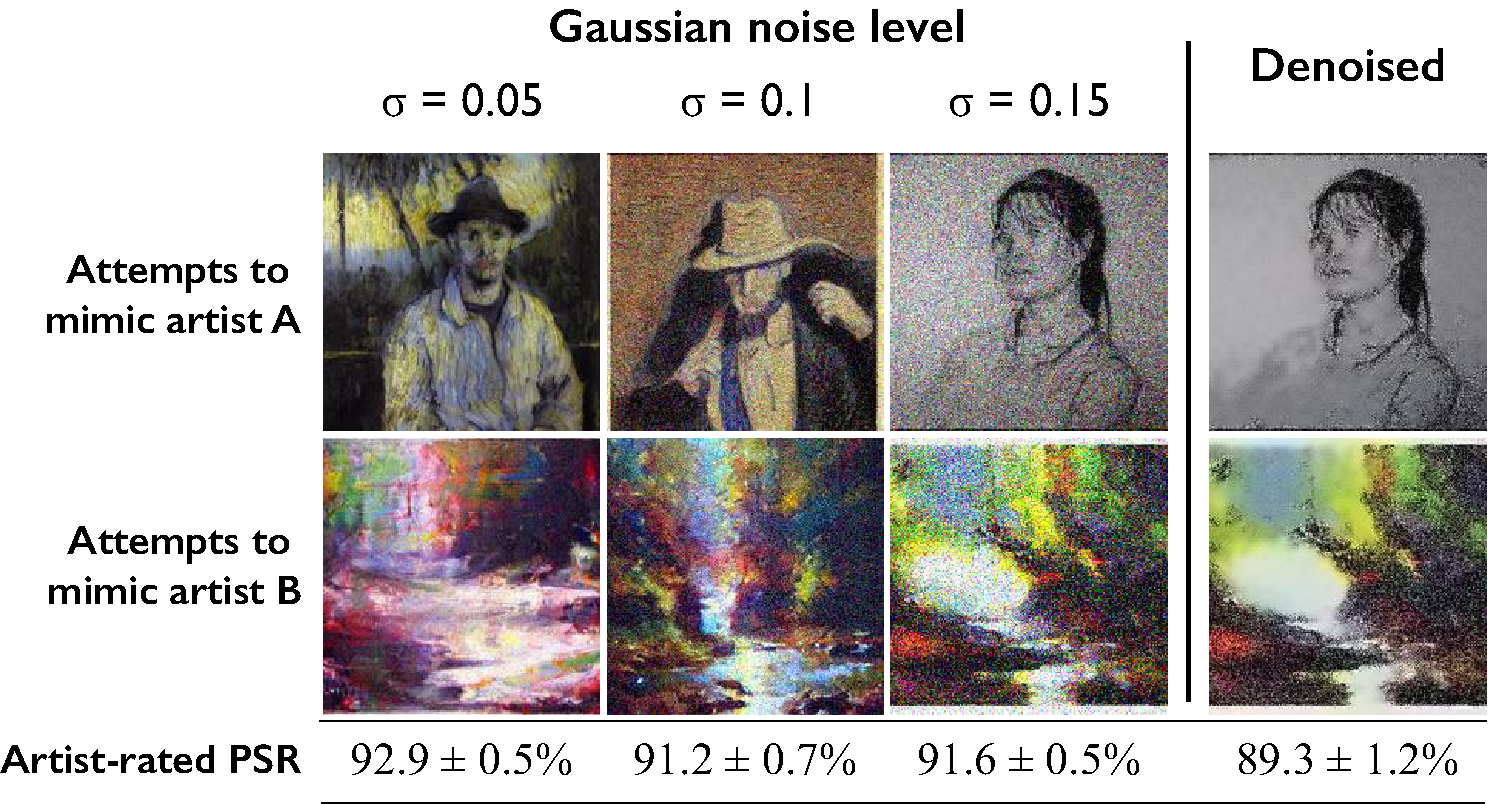
\includegraphics[width=1\columnwidth]{plots/counter/add-noise.pdf}
    \vspace{-0.25in}
  \caption{\system{}'s protection performance remains high as mimic adds an
    increasing amount of Gaussian noise to the cloaked artwork. Even when the
    mimic adds denoising (last column), \system{}'s protection persists. } 
  \label{fig:noise_countermeasure}
\end{figure}

\begin{figure}[t]
  \centering
  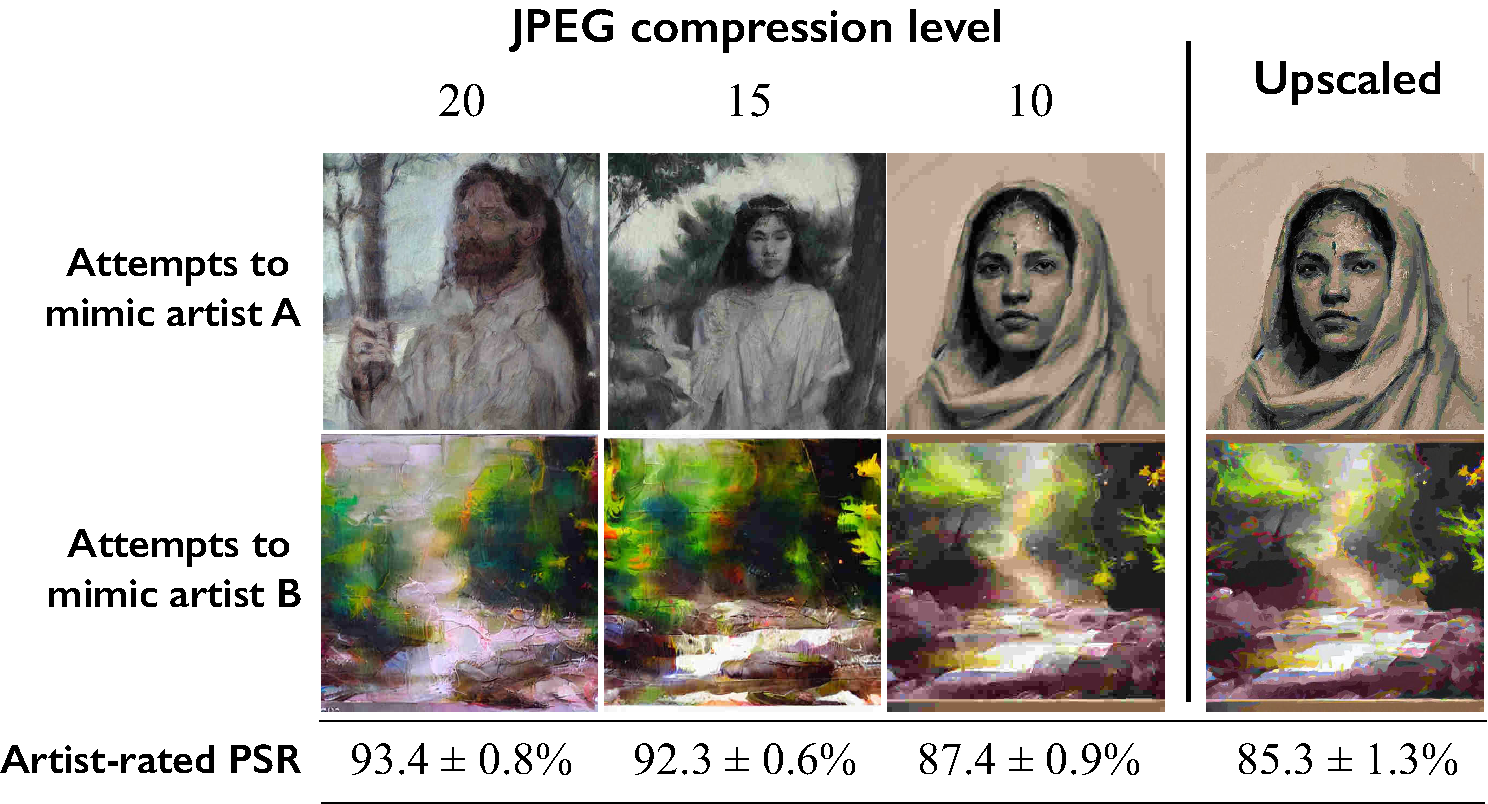
\includegraphics[width=1\columnwidth]{plots/counter/add-compression.pdf}
  \vspace{-0.25in}
  \caption{\system{}'s protection performance remains high as mimic adds JPEG compression to the cloaked artwork. Even when the mimic also upscales the mimicked images (last column), \system{}'s protection persists. }
  \label{fig:jpeg_countermeasure}
\end{figure}

\secspace
\section{Countermeasures} 
\label{sec:counter}

We consider potential countermeasures a mimic could employ to reduce the
effectiveness of \system. We consider the strongest adversarial setting, in
which the mimic has white-box access to our protection system, \ie access to
the feature extractor used and protection algorithm. In our experiments, we
assume the mimic uses the SD model as the generic model and test the efficacy
of each countermeasure on the $13$ victim artists from
\S\ref{sec:metrics}. Here, we focus on artist-rated PSR metric, because many
countermeasures trade off image quality for mimicry efficacy, and
CLIP-based metric does not consider image quality.

\para{Image transformation. } A popular approach to mitigate the impact of
small image perturbations, like those introduced by \system{}, is to
transform training images before using them for model
training~\cite{carlini2017adversarial,feinman2017detecting}. In our setting,
the mimic could augment the cloaked artwork before fine-tuning their model on
them to potentially reduce cloak efficacy. We first test \system{}'s
resistance to two popular image transformations, adding Gaussian noise and
image compression. We also consider a stronger version of this countermeasure
that then tries to correct the image quality degradation introduced by the
transformations.

Transforming cloaked artwork does not defeat \system{}'s
protection. Figure~\ref{fig:noise_countermeasure} shows that as the magnitude
of Gaussian noise ($\sigma$) increases, the quality of mimicked artwork
decreases as fast as or faster than cloak effectiveness. This is because
models trained on noisy images learn to generate noisy images. We observe a
similar outcome when mimic uses JPEG compression
(Figure~\ref{fig:jpeg_countermeasure}), where image resolution and quality
degrade due to heavy compression. Artists-rated PSR decreases slightly but
remains above $>87.4\%$ across both types of data transformations. Artists
consider \system{}'s protection to be successful when mimicked artwork is of
poor quality.  

The mimic can take this countermeasure one step further by \textit{reversing}
the quality degradation introduced by the noising/compression
process. Specifically, a mimic can run image denoising or image upscaling
tools on the mimicked artwork (\eg ones shown in
Figure~\ref{fig:noise_countermeasure} and \ref{fig:jpeg_countermeasure}) to
increase their quality. We found this approach improves generated image
quality but still does not allow for successful mimicry. For denoising, we
ran a state-of-the-art CNN-based image denoiser~\cite{zhang2017beyond} that
is specifically trained to remove ``additive Gaussian noise'' (the same type
of noise added to cloaked artwork). The last column of
Figure~\ref{fig:noise_countermeasure} shows the denoised image (using the
noisy mimicked image when $\sigma=0.2$ as the input). While the process
removes significant amounts of noise, the denoised artwork still has many
artifacts, especially around complex areas of the artwork (\eg human
face). We observe similar results for image upscaling, where we use a
diffusion-based image upscaler~\cite{stable2-1} to improve the quality of
compressed images (Figure~\ref{fig:jpeg_countermeasure}). Overall, our
artist-rated protection success rate remains $> 85.3\%$ against this improved
countermeasure.  

\begin{figure}[t]
  \centering
  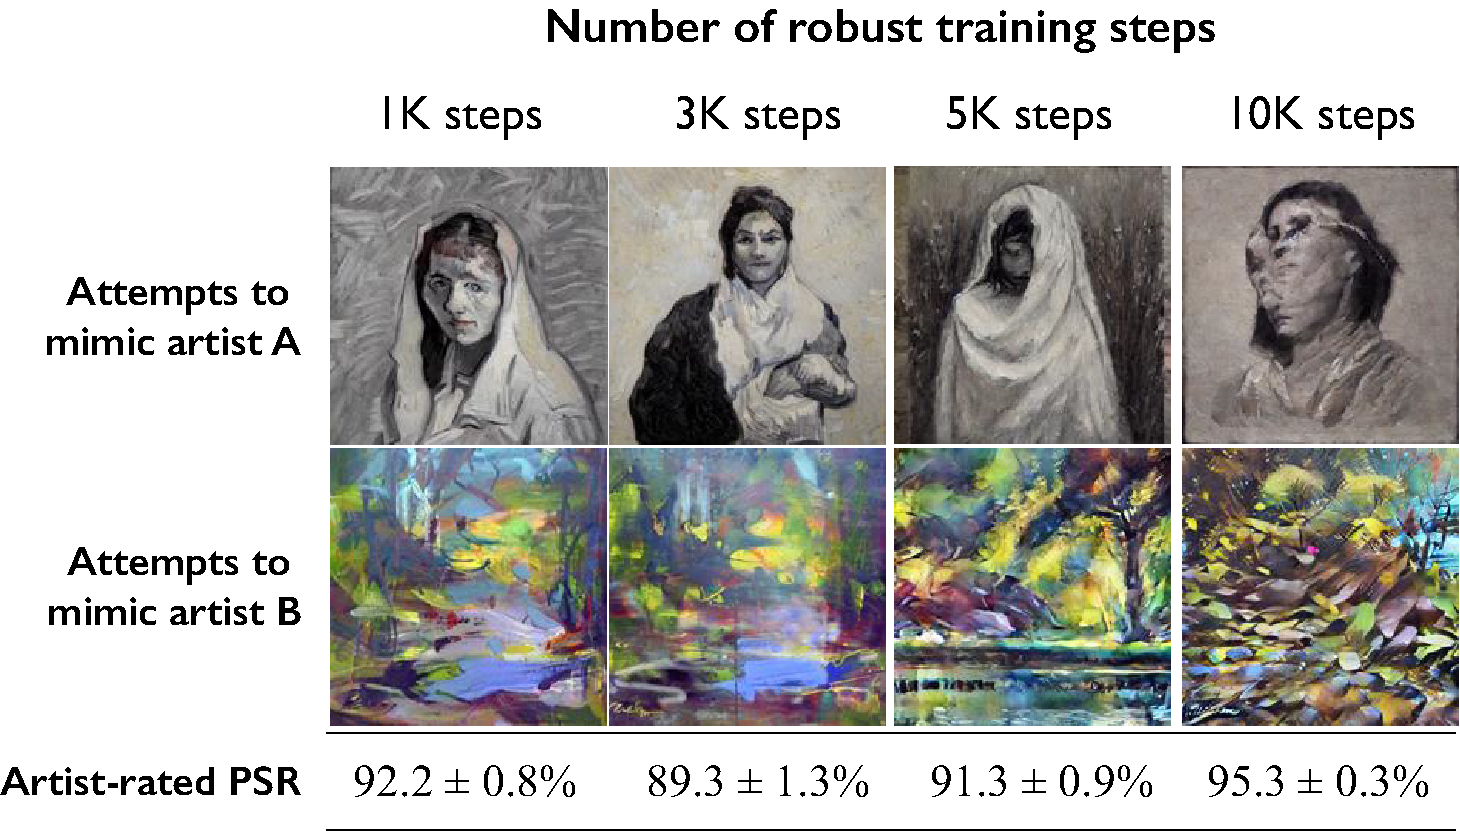
\includegraphics[width=1\columnwidth]{plots/counter/florian.pdf}
  \caption{\system{}'s protection performance remains high against robust training countermeasure proposed by Radiya \etal. The protection performance first decreases then increases as mimic robustly trains the model with an increasing number of steps. }
  \label{fig:florian}
\end{figure}

\para{Radiya \etal~\cite{radiya2021data} robust training.} Radiya
\etal~\cite{radiya2021data} design a robust training method to defeat
cloaking tools like Fawkes~\cite{shan2020fawkes} and
Lowkey~\cite{cherepanova2021lowkey} in the face recognition setting. At a
high level, this method augments the attacker's training dataset with some
cloaked images generated by the cloaking tool and the \textit{correct} output
labels. Training on such data makes the model more robust against cloak
perturbations on unseen cloaked images at inference time, and thus, can
potentially circumvent the protection.
% Radiya \etal further proposed an add-on method to prevent degrading the normal classification accuracy on \textit{uncloaked images}, but this add-on does not impact the classification on cloaked data.
%More details about this countermeasure can be found in~\cite{radiya2021data}. 

% To avoid degrading classification accuracy on benign inputs, a well-known drawback of adversarial training, Radiya \etal further propose to use ``confidence thresholding'', which only uses a robust model for classification if a non-robust model, which runs first, has low confidence in its classification. While increases the classification accuracy on unprotected data, ``confidence thresholding'' does not impact the classification accuracy on cloaked data. 

% We apply a similar confidence thresholding method to maintain mimickry performance when plagiarizing unprotected artist. But for artists protected by \system, mimic has to use the robust model to mimic their styles. 
We test if this robust training approach can defeat \system{}. We assume the
mimic first robustly trains the feature extractors in their generic models
using cloaked artwork generated by \system{}, and then trains the generator
model to generate images from the robust feature space. Finally, the mimic
uses the robust generic model for style mimicry as in
\S\ref{sec:eval-cloak}. We discuss the detailed robust training setup in
Appendix~\ref{app:counter}.  

\system{} performance remains high, even if the mimic robustly trains the
generic model for many iterations before using it for style mimicry (see
Figure~\ref{fig:florian}). As the model becomes more robust, the mimicked
artwork is less impacted by cloaking (less influenced of the target
style). However, robust training greatly degrades mimicked image quality,
preventing successful mimicry. Overall, the artist-rated PSR remains
$>~88.7\%$. To mitigate robust training's impact on image quality, we explore
an alternative robust training method, where we robustly train a new feature
extractor designed to remove cloak's impact while operating in the
original feature space (thus no need to change the image
generator). We found this robust training approach is also ineffective
(details in \S\ref{app:counter}).

As discussed in \S\ref{sec:cloak-effect}, \system{} remains reasonably
effective against Radiya \etal because 1) the continuous output space of the
generative model, and 2) high quality requirement of art generation. Robust
training reduces cloaking's effectiveness but cannot completely remove its
impact. In the classification case (facial recognition), this reduced
effectiveness only manifests in small changes in classification confidence
(compared to no cloaking) and often does not change the discrete classification
outcome. However, in the context of generator models, the continuous output space means
that even less-effective cloaks still directly affect the mimicked
artwork. Combined with the high quality requirement, the reduced protection
effect is enough to disrupt style mimicry, as shown in
Figure~\ref{fig:florian}. Additional robust training simply degrades
generation quality, rather than reducing cloaking efficacy.


\revise{
  
\para{Outlier Detection. } Another countermeasure could involve
leveraging outlier detection to identify and remove protected images~\cite{wang2021understanding,shan2020gotta,wang2019neural}. We
test \system{}'s robustness to a state-of-the-art outlier detection method that leverages
contrastive training~\cite{wang2021understanding}. Contrastively trained
models project data into a well-separated feature space, which the mimic
could leverage. 

We assume the mimic has a ground truth set (20) of original artworks from a
given artist. The mimic first projects these art pieces into the feature space
of a model trained with contrastive loss on ImageNet
dataset~\cite{wang2021understanding}. The mimic then trains a one-class SVM
outlier detector~\cite{li2003improving} using these ground truth
features. Now, given a new artwork from the same artists, the mimic detects
whether the artwork is an outlier using the detector. Detection results on
$4$ current artists (\S\ref{sec:eval-cloak}) show that outlier detection has
limited effectiveness against \system{} ($< 65\%$ precision and $< 53\%$
recall at detecting \system{} protected images).  
}



